\subsection{ECHO model (model ID: 44)}
The ECHO model (fig.~\ref{fig:44_schematic}) is a single element from the Spatially Explicit Hydrologic Response (SEHR-ECHO) model \citep{Schaefli2014}. Because the model is used as a lumped model here, the "SEHR" prefix was dropped intentionally. For consistency with other models, soil moisture storage $S$ is given here in absolute terms [mm], rather than fractional terms that are used in the original reference. Rain- and snowfall equations are taken from \citet{Schaefli2005}. The model has 6 stores and 16 parameters ($\rho$, $T_s$, $T_m$, $a_s$, $a_f$, $G_{max}$, $\theta$, $\phi$, $S_{max}$, $sw$, $sm$, $K_{sat}$, $c$, $L_{max}$, $k_f$ and $k_s$). The model aims to represent:

\begin{itemizecompact}
\item Interception by vegetation;
\item Snowfall, snowmelt, ground-heat flux and storage and refreezing of liquid snow;
\item Infiltration, infiltration excess and saturation excess;
\item Fast and slow runoff.
\end{itemizecompact}

\subsubsection{File names}
\begin{tabular}{@{}ll}
Model: &m\_44\_echo\_16p\_6s \\
Parameter ranges: &m\_44\_echo\_16p\_6s\_parameter\_ ranges \\
\end{tabular}

% Equations
\subsubsection{Model equations}

% Model layout figure
{ 																	% This ensures it doesn't warp text further down
\begin{wrapfigure}{l}{5cm}
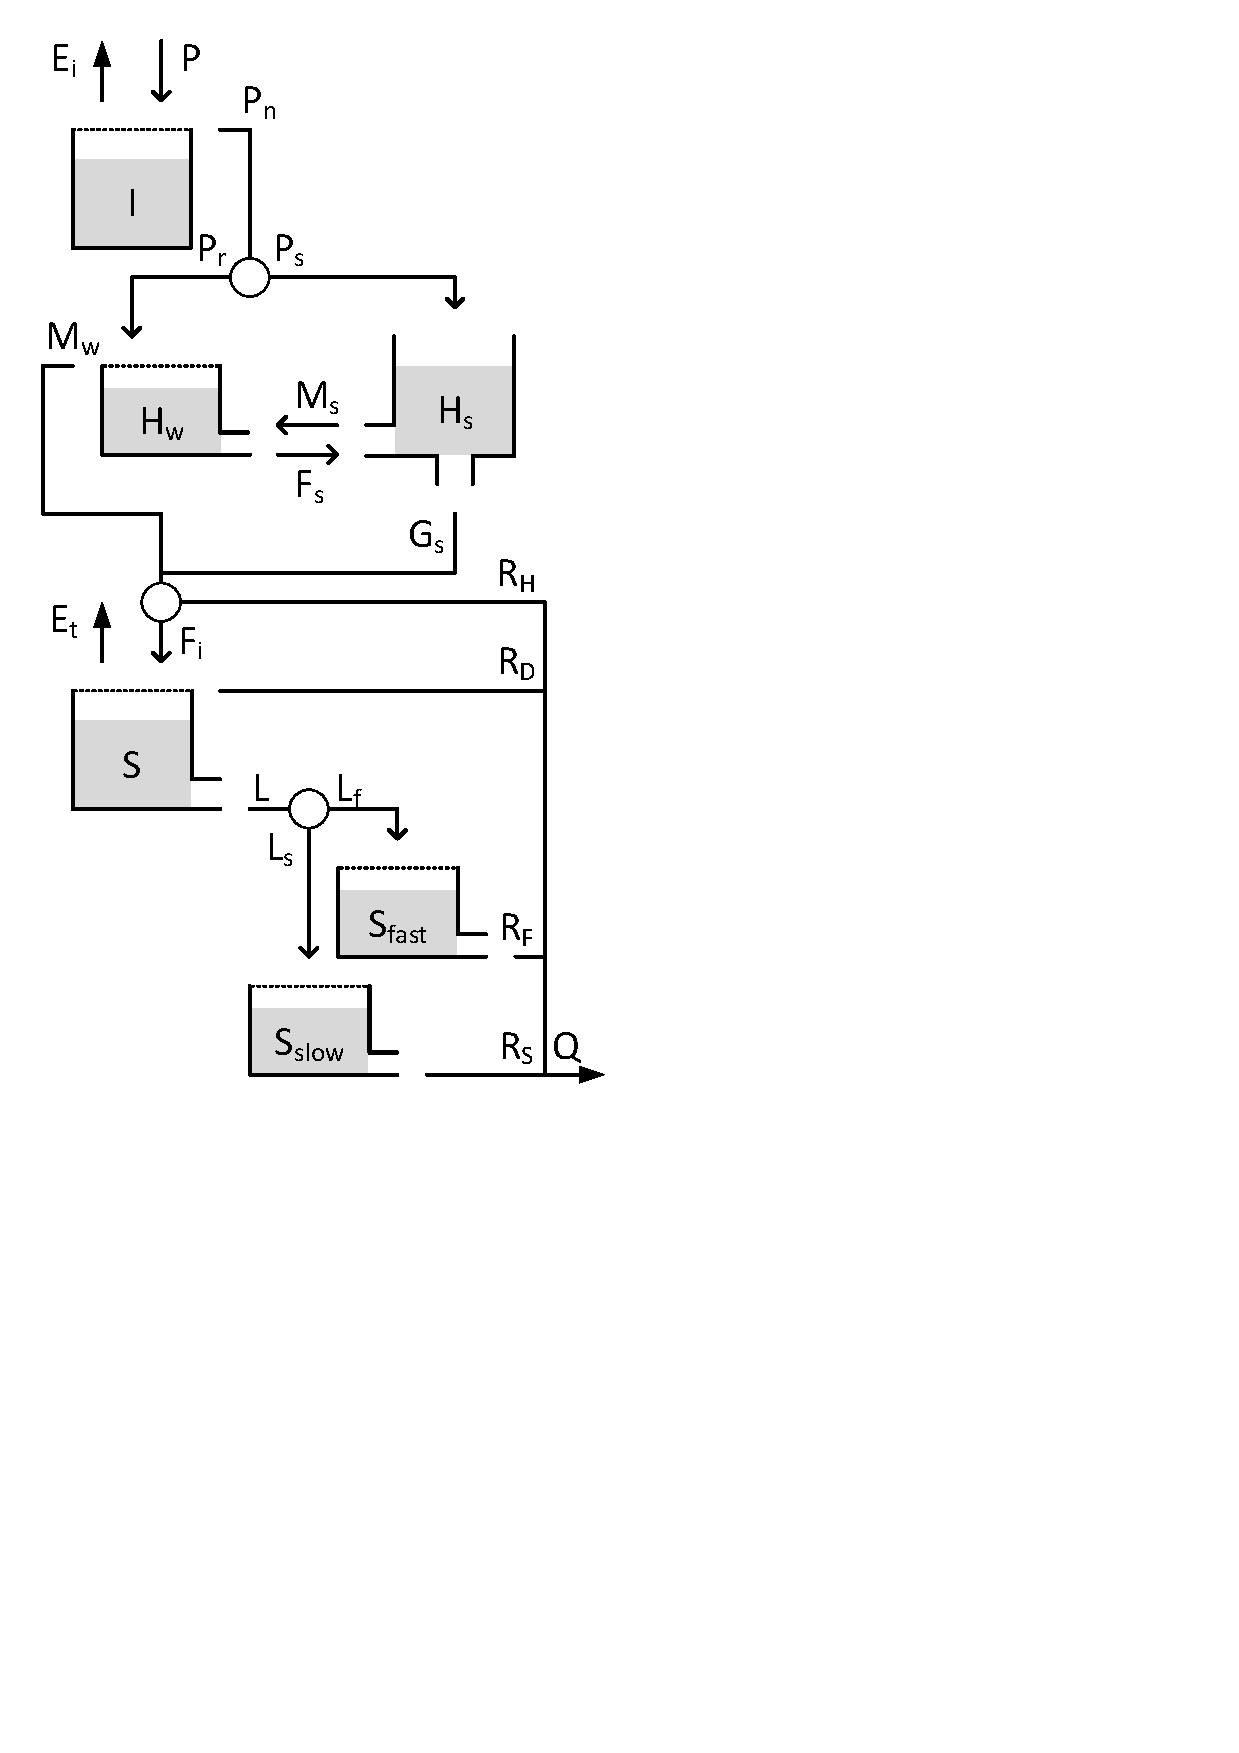
\includegraphics[trim=1cm 11cm 7cm 1cm,width=7cm,keepaspectratio]{./files/44_schematic.pdf}
\caption{Structure of the ECHO model} \label{fig:44_schematic}
\end{wrapfigure}

\begin{align}
	\frac{dI}{dt} &= P-E_i-P_n \\
	E_i &= \begin{cases}
		E_p, &\text{if } I >0 \\
		0, & \text{otherwise} \\
	\end{cases} \\
	P_n &= 
	\begin{cases}
		P, & \text{if } I = \rho \\
		0, & \text{otherwise}
	\end{cases}
\end{align}

Where $I$ [mm] is the current interception storage, refilled by precipitation $P$ $[mm/d]$ and drained by evaporation $E_i$ $[mm/d]$ and net precipitation $P_n$ $[mm/d]$.
$E_i$ occurs at the potential rate $E_p$ $[mm/d]$ when possible. 
$P_n$ only occurs when the store is at maximum capacity $\rho$ [mm].

} % end of wrapfigure fix

\begin{align}
	\frac{dH_s}{dt} &= P_s + F_s - M_s - G_s\\
	P_s &= \begin{cases}
		P_n, &\text{if } T \leq T_s \\
		0, & \text{otherwise} \\
	\end{cases} \\
	M_s &= \begin{cases}
		a_s(T-T_m), &\text{if } T > T_m, H_s > 0 \\
		0, &\text{otherwise}\\
	\end{cases}	\\
	F_s &= \begin{cases}
		a_fa_s(T_m-T), &\text{if } T < T_m, H_w > 0 \\
		0, &\text{otherwise}\\
	\end{cases} \\
	G_s &= \begin{cases}
		G_{max}, &\text{if } H_s > 0 \\
		0, &\text{otherwise} \\
	\end{cases} 
\end{align}

Where $H_s$ [mm] is the current storage in the snow pack, refilled by precipitation-as-snow $P_s$ $[mm/d]$ and refreezing of melted snow $F_s$ $[mm/d]$, and drained by snowmelt $M_s$ $[mm/d]$ and the ground-heat flux $G_s$ $[mm/d]$.
$P_s$ is calculated as all effective rainfall after interception, provided the temperature is below a threshold $T_s$ $[^oC]$.
$M_s$ uses a degree-day factor $a_s$ $[mm/^oC/d]$ and threshold temperature for snowmelt $T_m$ $[^oC]$.
$F_s$ occurs if the current temperature is below $T_m$ and the degree-day rate reduced by factor $a_f$ [-].
$G_s$ occurs at a constant rate $G_{max}$ $[mm/d]$.

\begin{align}
	\frac{dH_w}{dt} &= P_r +M_s-F_s-M_w \\
	P_r &= \begin{cases}
		P_n, &\text{if } T > T_s \\
		0, & \text{otherwise} \\
	\end{cases} \\
	M_w &=\begin{cases}
		P_r + M_s, &\text{if } H_w = \theta*H_s \\
		0, & \text{otherwise} \\
	\end{cases} 
\end{align}
  
Where $H_w$ [mm] is the current storage of liquid water in the snow pack, refilled by precipitation-as-rain $P_r$ $[mm/d]$ and snowmelt $M_s$ $[mm/d]$, and drained by refreezing $F_s$ $[mm/d]$ and outflow of melt water $M_w$ $[mm/d]$.
$P_r$ is calculated as all effective rainfall after interception, provided the temperature is above a threshold $T_s$ $[^oC]$.
$M_w$ occurs only if the store is at maximum capacity, which is a fraction $\theta$ [-] of the current snow pack height $H_s$ [mm].

\begin{align}
	\frac{dS}{dt} &= F_i - R_D -E_t -L \\
	F_i &= P_{eq} - R_H\\
	P_{eq} &= M_w+G_s\\
	R_H &= \begin{cases}
		max(P_{eq}-\phi,0), &\text{if } S < S_{max} \\
		0, & \text{otherwise} \\
	\end{cases} \\
	R_D &= \begin{cases}
		P_{eq}, &\text{if } S = S_{max} \\
		0, & \text{otherwise} \\
	\end{cases} \\
	E_t &= min\left(max\left(0,E_{t,pot}\frac{S-sw}{sm -sw}\right), E_{t,pot}\right)\\
	E_{t,pot} &= E_p - E_i\\
	L &= K_{sat}S^c
\end{align}

Where $S$ [mm] is the current storage in the soil moisture zone, refilled by infiltration $F_i$ $[mm/d]$ and drained by Dunne-type runoff $R_D$ $[mm/d]$, evapotranspiration $E_t$ $[mm/d]$ and leakage $L$ $[mm/d]$.
$F_i$ is calculated as equivalent precipitation $P_{eq}$ minus Horton-type runoff $R_H$. 
$P_{eq}$ is the sum of melt water $M_w$ and the ground-heat flux $G_s$. 
$R_H$ occurs at fixed rate $\phi$ $[mm/d]$ and only if the soil moisture is not saturated.
$R_D$ is equal to equivalent precipitation $P_{eq}$ but occurs only when the store is at maximum capacity $S_{max}$ [mm].
$E_t$ fulfils any leftover evaporation demand after interception. 
$ E_t$ occurs at the potential rate until the plant stress point $sm$ [mm], decreases linearly until the wilting point $sw$ [mm] and is zero for any lower storage values.
$L$ has a non-linear relationship with storage through time parameter $K_{sat}$ $[d^{-1}]$ and coefficient $c$ [-].

\begin{align}
	\frac{S_{fast}}{dt} &= L_f - R_f\\
	L_f &= L-L_{s} \\
	L_s &= min(L,L_{max}) \\
	R_f &= k_f * S_{fast} 
\end{align}

Where $S_{fast}$ [mm] is the current storage in the fast runoff reservoir, refilled by leakage-to-fast-flow $L_f$ $[mm/d]$ and drained by fast runoff $R_f$ $[mm/d]$.
$L_f$ depends on leakage $L$ from soil moisture and the leakage-to-slow-flow $L_s$. 
$L_s$ is calculated from a maximum leakage rate $L_{max}$ $[mm/d]$.
$R_f$ has a linear relation with storage through time parameter $k_f$ $[mm/d]$.

\begin{align}
	\frac{dS_{slow}}{dt} &= L_s - R_s \\
	R_s &= k_s * S_{slow} 
\end{align}

Where $S_{slow}$ [mm] is the current storage in the slow runoff reservoir, refilled by leakage-to-slow-flow $L_s$ $[mm/d]$ and drained by slow runoff $R_s$ $[mm/d]$.
$R_s$ has a linear relation with storage through time parameter $k_s$ $[mm/d]$.
Total flow:

\begin{align}
	Q &= R_H+R_D+R_F+R_S
\end{align}

\subsubsection{Parameter overview}
% Table generated by Excel2LaTeX from sheet 'Sheet1'
\begin{table}[htbp]
  \centering
    \begin{tabular}{lll}
    \toprule
    Parameter & Unit  & Description \\
    \midrule
    $\rho$ & $mm$  & Maximum interception storage \\
    $T_s$ & $^oC$ & Threshold temperature for snowfall \\
    $T_m$ & $^oC$ & Threshold temperature for snowmelt \\
    $a_s$ & $mm~^oC^{-1}~d^{-1}$ & Degree-day factor for snowmelt \\
    $a_f$ & $-$   & Degree-day factor reduction factor for refreezing \\
    $G_{max}$ & $mm~d^{-1}$ & Snow melt through ground heat flux rate \\
    $\theta$ & $-$   & Water holding capacity as fraction of current snow pack \\
    $\phi$ & $mm~d^{-1}$ & Maximum Horton type flow rate \\
    $S_{max}$ & $mm$  & Maximum soil moisture storage \\
    $sw$  & $mm$  & Wilting point \\
    $sm$  & $mm$  & Plant stress point \\
    $K_{sat}$ & $d^{-1}$ & Runoff coefficient \\
    $c$   & $-$   & Runoff non-linearity \\
    $L_{max}$ & $mm~d^{-1}$ & Maximum leakage rate \\
    $k_f$ & $d^{-1}$ & Runoff coefficient \\
    $k_s$ & $d^{-1}$ & Runoff coefficient \\
    \bottomrule
    \end{tabular}%
  \label{tab:addlabel}%
\end{table}%

